\chapter{Methods}
\label{chap:methods}
\khExplicitPfalse
\graphicspath{{/home/ram/Desktop/Acads/Phd/dissertation/psuThesis/Chapter-2/Figures/}{/usr/users/rsubrama/Desktop/Acads/Phd/dissertation/psuThesis/Chapter-2/Figures/}}
    As mentioned in Sec. \ref{sec:chap1VirialCoefficients} the number of configuration integrals to be evaluated increases exponentially with the order of virial coefficient. In addition to that, the use of \abinitio{} potentials for quantum virial coefficient calculations involve siginificantly more computational effort than simple potential models. The need for such high quality virial coefficients, in order to predict accurate theromdynamic properties, should not be underestimated. Therefore efficient techniques are required in order to perform virial coefficient calculations. Graph theoretical methods were needed to represent the integrals as diagrams with a weight associated to it, especially for higher order coefficients, where writing out the integral would prove to be cumbersome. On the one hand, there have been theoretical methods \cite{Ree1964,Hellmann2011} developed to either reduce the number of these diagrams or combine them in a concise manner so as to improve the computational efficiency. On the other, computational techniques such as the VEGAS algorithm \cite{Lepage1972}, Mayer Sampling Monte Carlo (MSMC) \cite{Singh2004} and Wheatley's algorithm \cite{Wheatley2013} have also been developed to evaluate a given set of diagrams efficiently. The different theoretical methods and computational techniques complement each other very well and have made possible, for instance, the calculation of 16$^{\text{th}}$-order virial coefficents for the Lennard Jones model \cite{Feng2015}. Since the main aim of this work was to develop efficient methods, we shall restrict our attention to MSMC algorithm and the evaluation of second and third quantum virial coefficients for different systems. In that spirit, we present a brief summary of the MSMC algorithm in the following section.

\section{Mayer Sampling Monte Carlo}
    \label{sec:MSMC}
    \subsection{Introduction}
    \label{subsec:MSMCintro}
    MSMC is a free-energy perturbation technique which was developed by Singh and Kofke \cite{Singh2004} that involves avoiding the direct calculation of any desired integral (denoted as the `target') by computing its ratio to a known reference integral. The method uses importance sampling where the weight of a configuration is taken to be the absolute value of the integrand. Although it was developed originally using an umbrella-sampling \cite{Singh2004,Frenkel,Schultz2009} method, in its most recent form, the working equations of MSMC are cast using overlap-sampling method as:
    \begin{equation}
        \label{eq:MSMCworking}
        \begin{aligned}
            \Gamma (T) &= \Gamma_o \frac{{<\gamma/\pi>}_\pi / {<\gamma_{os}/\pi>}_\pi}{{<\gamma_o/\pi>}_{\pi_o} / {<\gamma_{os}/\pi_o>}_{\pi_o}}\\
            \gamma_{os} &= \frac{|\gamma_o||\gamma|}{\alpha |\gamma_o| + |\gamma|}
        \end{aligned}
    \end{equation}
    where $\Gamma (T)$ is the target integral, $\gamma$ is the target integrand, $\pi$ is the sampling weight of the target integrand, the subscript `$o$' denotes the corresponding quantities for the reference integral and integrands respectively, $\alpha$ is Bennett's \cite{Bennett1976} optimization parameter, and angular brackets $<\ldots>$ represent ensemble-averages.

    If computed directly, the target integral involves averaging lots of really large positive and negative numbers which could lead to imprecise results, especially for virial coefficient calculations \cite{Singh2004}. However, using MSMC this calculation is reduced to averaging the sign of the integrand because of the use of importance sampling, where we set $\pi = |\gamma|$. Thus, MSMC results in a more precise value than direct evaluation using numerical techniques. Additionally it is also computationally efficient than numerical techniques for higher order integrals. The versatility of the MSMC approach lies in the fact that it can be applicable to the evaluating of any integral irrespective of the its functional form (with a few caveats, for details see Ref. \cite{Singh2004}) with a whole variety of choices for the reference. For virial coefficient calculation purposes, $\Gamma$ is taken to be the configuration integral or sum of integrals. Singh and Kofke \cite{Singh2004} analyzed different options wih respect to calculating virial coefficents and suggested the use of hard-spheres as the reference for two reasons: 1) virial coefficients of hard spheres are temperature independent and 2) have been already evaluated precisely in literature. Highly precise and accurate virial coefficients of many systems including mixtures \hl{cite group papers here} have been successfully computed using MSMC, thus establishing a track-record of its performance. Hence, in all the computations performed related to this work, we have employed MSMC to compute virial coefficients efficiently.

    \subsection{Implementation}
    \label{subsec:MSMCimplementation}
        The idea behind this section is to outline some of the key features of a typical MSMC simulation that are common to all the systems, at the beginning, so that we need not repeat these for each type of system in later chapters. We may then focus on system-specific parameters within the `Computational details' section for each chapter. We provide details of how we collect data and our procedure to estimate the uncertainty as well.

        A typical MSMC simulation consists of two types of systems `target' and `reference'. Configurations are generated via MC trials for each system and are accepted/rejected with a probability $P_{\text{acc}}$:
        \begin{equation}
            \label{eq:MCacceptance}
            P_{\text{acc}} = \text{Min} \left(1, \displaystyle\frac{\pi^{\text{new}}}{\pi^{\text{old}}} \right)
        \end{equation}
        where $\pi$ is the sampling weight for that particular system, superscripts old and new are used to denote the old and new configurations respectively.

        Note that in Eq. \eqref{eq:MSMCworking}, ${<\gamma/\pi>}_\pi$ and ${<\gamma_{os}/\pi>}_\pi$ are called the target average and target-overlap average respctively. The corresponding terms for the reference system are called the reference average and the reference-overlap average respectively. In all MSMC simulations and for each system, molecule 0 always remains fixed at the origin and all MC trials generate configurations of the other molecules present in the system. A short equilibration simulation is performed at the beginning to determine $\alpha$ (Eq. \eqref{eq:MSMCworking}) and to adjust MC move step sizes so that the acceptance of all the MC moves is 50\%. Irrespective of their number, all MC moves are chosen with equal probability for both the systems within the simulation. After the equilibration period, we start collecting values of the reference, target, reference-overlap and target-overlap averages. The total number of configuration samples is divided into blocks of 1000 samples each. We compute averages of these four quantities and their standard deviation for each block. We then combine the averages across all blocks and use standard error formulas to estimate the overall value along with its standard deviations. The final values of virial coefficients and their standard deviations reported throughout this work are then obtained by using the reference, target, reference-overlap and target-overlap averages computed as mentioned above, Eq. \eqref{eq:MSMCworking} and simple error propagation formulas.

\section{Path Integrals}
    \subsection{Introduction}
        In this section we introduce the formalism developed by Richard Feynman \cite{Feynman} which provides guidelines for accounting nuclear quantum effects in quantum mechanical calculations. We do not attempt a fully rigorous mathematical re-derivation here but rather highlight some of they key aspects and formulas (from Feynman's book \cite{Feynman}) which are useful for the purpose of quantum virial coefficient calculations. For further details, the interested reader may refer Refs. \hl{PI references}. Primarily, the purpose of this section is to establish a relationship between the thermal density matrix which is derived from statistical mechanics and the kernel of the wave function derived from the \Schrodinger{} equation. Thus creating the important link between microscopic states and macroscopic observables.

        The advent of quantum mechanics in the 1920s brought about a fundamentally new way of thinking about relativistic particles. The classical definitions of probability due to Laplace could no longer be applicable for systems of extremely small sizes. Note that what had changed was not the idea or concept of probability but rather the prescribed way of computing it. Different physicists proposed different hypotheses for computing the probability according to quantum mechanics.

        Feynman's Path Integral (PI) formalism has at its beginning stages, simple probability definitions associated with events for a relativistic particle such as the electron. One important idea was to associate a complex amplitude ($\phi(x)$) with the probability of an event $P$ depending on some variable $x$, such that $P = |\phi(x)|^2$. Since there could be many possible ways for the event to happen, we associate an amplitude to each such alternative and compute the overall probability as $P = |\Phi(x)|^2; \Phi(x) = \phi_1(x) + \phi_2(x) + \cdots$. Similarly, expressions for events occuring in succession, mutually exclusive events and various other definitions corresponding to classical probability, can be obtained. Starting with these basic definitions, for each path or trajectory associated with the movement of a particle, a contribution to the probability amplitude was associated. Therefore, we could define a quantity called `kernel' that represented the sum of contributions from each possible path. The action $S$ associated with a particle of mass $m$ traveling in a potential $V(x,t)$ is given in terms of its Lagrangian $L$ as:
        \begin{equation}
        \label{eq:action}
            \begin{aligned}
                S &= \displaystyle \int_{t_a}^{t_b} L(\dot{x},x,t) dt,\\
                L(\dot{x},x,t) &= \frac{m{\dot{x}}^2}{2} - V(x,t).
            \end{aligned}
        \end{equation}

        Whereas only the path with the least action contributes to the classical trajectory, all paths contribute equally to the quantum trajectory and do so in different phases. This was another important idea that was employed in the development of PI formalism. Based on the above definitions, we can calculate the probability associated with the movement of a particle from point $a$ to $b$:
        \begin{equation}
        \label{eq:quantum probability}
            \begin{aligned}
                \phi(x,t) &= \text{const.} e^{iS[x(t)]/\hbar},\\
                \Rightarrow K[b,a] &= \displaystyle\sum\limits_{\text{all paths}} \phi[x(t)],\\
                P(b,a) &= {|K[b,a]|}^2.
            \end{aligned}
        \end{equation}
        where $K[b,a]$ is the kernel.

        Consider a particle of mass $m$ traveling in a potential $V(x,t)$, with action defined as in Eq. \eqref{eq:action}. We can construct the ``path integral'' analogous to the Riemann integral:
        \begin{equation}
            \begin{aligned}
                K[b,a] &= \displaystyle\lim_{\epsilon\,\to\ 0} \frac{1}{A}\int_{-\infty}^\infty\,\int_{-\infty}^\infty\,\cdots\,\int_{-\infty}^\infty e^{\frac{iS[b,a]}{\hbar}}\,\frac{dx_1}{A}\,\frac{dx_2}{A}\ldots\,\frac{dx_{N-1}}{A},\\
                A &= {\left( \displaystyle\frac{2\pi i \hbar \epsilon}{m} \right)}^{\frac{1}{2}}.
            \end{aligned}
        \end{equation}
        More compactly, it can be written in terms of the new path integral notation $\mc{D} x(t)$ as:
        \begin{equation}
        \label{eq:PI compact kernel}
            K[b,a] = \displaystyle \int_{a}^b e^{\frac{iS[b,a]}{\hbar}} \mc{D} x(t).
        \end{equation}
        For a more general case of having $N-1$ intermediate points between $a$ and $b$, the kernel is given as:
        \begin{equation}
            \begin{aligned}
                K[b,a] = \int_{x_{N-1}}\,\cdots\,\int_{x_2}\,\int_{x_1} &K[b,N-1]K[N-1,N-2]\,\ldots\\
                & \qquad K[i+1,i] \ldots K[1,a]\,dx_1\,dx_2\ldots dx_{N-1}
            \end{aligned}
        \end{equation}
        
        \subsubsection{Kernel of the Wave Function}
            Assume that the amplitude to arrive at any point $b = (x,t)$ irrespective of the starting point $a$, to be given by $\psi (x,t)$. It can be shown that $\psi (x,t)$ also has the same probability charecteristics as the kernel, i.e., $P = |\psi (x,t)|^2$ and we call $\psi (x,t)$ the wave function. Based on this definition, we could compute the wavefunction exactly at any future point if we know its exact value at any time $t$.

            The \Schrodinger{} equation is solvable by separation of variables in the speical case where we use a time-indpendent Hamiltonian:
            \begin{equation}
                \label{eq:psi}
                \begin{aligned}
                    \psi(x,t) &= \phi(x)e^{(-i/\hbar)Et},\\
                    \mc{H} \phi(x) &= E \phi(x).
                \end{aligned}
            \end{equation}

            Using orthonormal basis functions to represent $\psi(x,t)$ and given $t_b > t_a$, the kernel is given by:
            \begin{equation}
                \label{eq:kpsi}
                K[x_b,t_b;x_a,t_a] = \displaystyle\sum\limits_{n = 1}^\infty \phi_n(x_b){\phi^*_n(x_a)} e^{(-i/\hbar)E_n(t_b - t_a)}
            \end{equation}
            where $\phi^*(x)$ denotes the complex conjugate of the $\phi(x)$ and $E_n$ are the eigenvalues of Eq. \eqref{eq:psi}. It can be shown that the kernal in Eq. \eqref{eq:kpsi} also satisfies the \Schrodinger{} equation.

        \subsubsection{Thermal Density Matrix}
            From statistical mechanics, we know that at thermal equilibrium at a temperature $T$, the probability that a system exists in a state with energy $E$ is proportional to the Boltzmann factor $e^{-\beta E}$. Here $\beta = 1/k_\text{B} T$ and $k_\text{B}$ is the Boltzmann constant. Assuming non-degenerate states, the normalized probability distribution is given by:
            \begin{equation}
                \begin{aligned}
                    p_n &= \frac{1}{Z}e^{-\beta E_n}, \\
                    Z &= \displaystyle\sum\limits_n e^{-\beta E_n}.
                \end{aligned}
            \end{equation}
            
            Suppose 'A' is some property of interest, its mean value in the $n^{th}$ energy state and the corresponding statistical average for the whole system are computed as:
            \begin{equation}
                \begin{aligned}
                    A_n &= \displaystyle\int \phi_n^* A \phi_n d\Gamma,\\
                    \bar{A} &= \displaystyle\sum\limits_n p_n A_n = \frac{1}{Z} \displaystyle\sum\limits_n A_n e^{-\beta E_n}.
                \end{aligned}
            \end{equation}
            where $\Gamma$ denotes the configuration space and integral over $\Gamma$, the configurational integral.

            If the system exists in a single state defined by the wavefunction $\phi_n(x)$, the probability of observing it and the expectation value can be calculated as: 
            \begin{equation}
                \label{eq:prob stat mech}
                \begin{aligned}
                    P(x) &= \displaystyle\sum\limits_n \phi_n^*(x) \phi_n(x) e^{-\beta E_n}\\
                    \bar{A} &= \displaystyle \frac{1}{Z} \displaystyle\sum\limits_n A_n e^{-\beta E_n} = \frac{1}{Z} \displaystyle\sum\limits_n \int \phi_n^*(x) A \phi_n(x)\: e^{-\beta E_n} dx
                \end{aligned}
            \end{equation}

            We can calculate the expected value of any quantity A using if we know the function:
            \begin{equation}
                \label{eq:rho stat mech}
                \rho(x',x) = \displaystyle \sum\limits_n \phi_n(x') \phi_n^*(x) e^{-\beta E_n}
            \end{equation}
            
            From Eqs. \eqref{eq:prob stat mech} and \eqref{eq:rho stat mech}, we can write down the expression for the partition function $Z$ as:
            \begin{equation}
                \begin{aligned}
                    P(x) &= \frac{1}{Z} \rho(x,x),\\
                    Z &= \int \rho(x,x) dx \equiv \text{trace} \{\rho\}.
                \end{aligned}
            \end{equation}
            where $\rho(x',x)$ is called the statistical thermal density matrix at temperature T.
            
            Comparing the expressions for the kernel (Eq. \eqref{eq:kpsi}) and the density matrix (Eq. \eqref{eq:rho stat mech}), we see that if we replace `$t_b - t_a$' of Eq. \eqref{eq:kpsi} with `$-i \beta \hbar$' , the resulting expressions are identical. Therefore we can write:
            \begin{equation}
                \rho (x_b, x_a; \tau) = \displaystyle \int exp \left\{ - \frac{1}{\hbar} \: \int_0^{\tau} \left[ \frac{m}{2} {\dot{x}(u)}^2 + V(x(u)) \right] du \right\} \mc{D}x(u)
            \end{equation}
            where $\tau = \beta \hbar$, has units of time and this led to the often used expression `imaginary-time' path integrals. 
            
    \subsection{Path Integral Monte Carlo}
        The thermal density matrix $\rho$ plays a key role in Feynman's imaginary-time PI formalism and its application in Monte Carlo (MC) algorithms to compute physical properties of interest. In position space, it is given by \cite{Feynman,Ceperley1995,Cui1997}:
        \begin{equation}\label{eq:rho}
            \rho (R , R' ; \beta) = < R | e^{- \beta \ham{H} } | R' >
        \end{equation}
        where $R = \{\bm{r}_1, \bm{r}_2, \ldots \bm{r}_n\}$ and $\beta = 1/k_{\rm B}T$, with $k_{\rm B}$ Boltzmann's constant and $T$ the temperature. A key property of the density matrix is that the product of two density matrices is also a density matrix:
        \begin{equation}\label{eq:dmProduct}
            \rho (R, R'; \beta_1) \times \rho (R, R'; \beta_2) = \rho (R, R'; \beta_1 + \beta_2)
        \end{equation}
        This is because any operator (specifically the Hamiltonian operator \ham{H} here) is commutative with any scalar multiple of itself. This exact property allows us to write down the following $(P-1)$-fold convolution:
        \begin{equation}\label{eq:convolution}
            \rho (R_0, R_P; \beta) = \displaystyle\int \cdots \int dR_1 \, dR_2 \, \ldots \, dR_{P-1} \: \rho (R_0, R_1; \tau) \rho (R_1, R_2; \tau) \ldots \rho (R_{P-1}, R_P; \tau)
        \end{equation}
        where $\tau = \beta/P$. Note that even though the above expression is exact, one needs to make approximations to the thermal density matrix in order to compute the convolution efficiently. The simplest of the approximations is to assume that the kinetic-energy operator (\ham{T}) and the potential-energy operator (\ham{V}) in the Hamiltonian commute with each other. As $\tau \to 0$ or equivalently as $PT \to \infty$, the ``primitive approximation'' is given by:
        \begin{equation}\label{eq:primitiveApprox}
            e^{- \tau (\ham{T} + \ham{V})} \approx e^{- \tau \ham{T}} e^{- \tau \ham{V}}
        \end{equation}
        The Trotter formula proves that this approximation does converge to the right result in the $P \to \infty$ limit and is given by:
        \begin{equation}\label{eq:trotter}
            e^{- \beta (\ham{T} + \ham{V})} = \lim_{P \to \infty} \Big[ e^{- \tau \ham{T}} e^{- \tau \ham{V}} \Big]^P
        \end{equation}

        \subsubsection{Fully Quantum Second Virial Coefficients}
            In this section we provide expressions (without going into too much mathematical detail, for further information see Refs. \cite{Cui1997,Patkowski2008,Garberoglio2009,Garberoglio2014}) for the fully quantum virial coefficients, first for the case of a diatomic rigid rotor. The expression for the monatomic molecule can then be obtained simply by ignoring the terms related to the orientational degrees of freedom in it.

            Let $m$ and $I$ denote the mass of the atom and moment of interia of the rigid rotor respectively with $\Lambda_m = h/\sqrt{2\pi m k_B T}$. Its Hamiltonian is given by:
            \begin{equation}
            \label{eq:hDiatomic}
                \hat{h}_2 = \displaystyle\frac{\hat{\mbf{p}}^2}{2m} + \frac{\hat{\mbf{J}}_1^2}{2I} + \frac{\hat{\mbf{J}}_2^2}{2I} + \hat{U}(r,\Omega_1,\Omega_2)
            \end{equation}
            where $\hat{\mbf{p}}$ is the momentum operator conjugated to the COM separation, $\hat{\mbf{J}}_1$ and $\hat{\mbf{J}}_2$ are the angular momentum operators, $\hat{U}(r,\Omega_1,\Omega_2)$ is the intermolecular potential function in terms of the COM distance $r$ and the orientation vectors $\Omega_1$ and $\Omega_2$.

            Note that because the momentum operator is conjugated to the COM separation, we can use the set of vectors $\mbf{x}^i,\mbf{\Omega}_1^i, \mbf{\Omega}_2^i$ to denote the configuration of the two $i^\text{th}$ rigid rotors. Employing the primitive approximation (Eq. \eqref{eq:primitiveApprox}) to the diatomic Hamiltonian and using the Trotter formula \ref{eq:trotter}, we get \cite{Cui1997}:
            \begin{equation}
                \begin{aligned}
                    \left< \mbf{x}^i \left| \exp \left(-\displaystyle\frac{\beta \hat{\mbf{p}}^2}{2 m P} \right) \right| \mbf{x}^{i+1} \right> &= \displaystyle\frac{P^{3/2}}{\Lambda^3} \exp \left(-\displaystyle\frac{\pi P (\mbf{x}^i - \mbf{x}^{i+1})^2}{\Lambda_m^2}\right)\\
                    \left< \Omega^i \left| \exp \left(-\displaystyle\frac{\beta \hat{\mbf{J}}^2}{2IP} \right) \right| \Omega^{i+1} \right> &= \displaystyle\sum_{j=0}^\infty \frac{2j+1}{4 \pi} \mc{P}_j (cos (\theta_{i,i+1}))\nonumber \exp \left[-\beta j(j+1) \Upsilon/ P \right]
                \end{aligned}
            \end{equation}
            where $j$ is the angular quantum number, $\theta_{i,i+1}$ is the angle between bead orientation vectors $\Omega_i, \Omega_{i+1}$ and $\mc{P}_j$ is the Legendre polynomial of order $j$.

            Defining $\mbf{r} \equiv \mbf{x}^{(1)}, \mbf{\Delta}^{(i)} \equiv \mbf{x}^{(i+1)} - \mbf{x}^{(i)}$ and $\bar{U}$ as:
            \begin{equation}
                \label{eq:uBarDiatomic}
                \exp [-\beta \bar{U} (|\mbf{r}|) = \left< \exp \left[ -\displaystyle\frac{\beta}{P} \sum_{i=1}^P U (|\mbf{x}^i|,\Omega_1^i,\Omega_2^i) \right] \right>_{F,\varrho}
            \end{equation}
            where $<\cdots>_{F,\varrho}$ denotes the ensemble average over ring polymer conformations $\mbf{\Delta}$ and rotor orientations $\mbf{\Omega}_1$ and $\mbf{\Omega}_2$ sampled according to the distributions $F$ and $\varrho$ defined below:
            \begin{subequations}
                \begin{align}
                    F(\mbf{\Delta}) &= \Lambda_m^3 { \left( \frac{P^{3/2}}{\Lambda_m^3} \right)}^P \exp \left( - \frac{\pi P}{\Lambda_m^2} \displaystyle\sum\limits_{i=1}^P {|\mbf{\Delta}^{(i)}|}^2 \right)\label{eq:fRingDiatomic}\\
                    \varrho(\mbf{\Omega}) &= \frac{1}{q_{rot}} \displaystyle\prod_{i=1}^P \sum_{j=0}^\infty \frac{2j+1}{4 \pi} \mc{P}_j (cos (\theta_{i,i+1})) \exp \left[-\beta j(j+1) \Upsilon/ P \right],\label{eq:rhoDiatomic}\\
                    q_{rot} &= \displaystyle\sum_{l} (2l + 1) \exp \left[-\beta \Upsilon l (l+1) \right],\nonumber\\
                    \Upsilon &= \displaystyle\frac{\hbar^2}{2I}\nonumber.
                \end{align}
            \end{subequations}

            The fully quantum second virial coefficient based on $\bar{U} (r)$ (Eq. \eqref{eq:uBarDiatomic}), for a diatomic molecule is given by:
            \begin{equation}
            \label{eq:b2Diatomic}
                B_2 (T) = -2 \pi \displaystyle\int dr~ r^2 (e^{-\beta \bar{U} (r)} - 1)
            \end{equation}

            To obtain the the expression for the case of the monatomic molecule, we simply ignore all the orientation related terms to obtain:
            \begin{equation}
                \label{eq:uBarMonatomic}
                \exp [-\beta \bar{U} (|\mbf{r}|) = \left< \exp \left[ -\displaystyle\frac{\beta}{P} \sum_{i=1}^P U (|\mbf{x}^i|) \right] \right>_F
            \end{equation}
            where $<\cdots>_F$ denotes the ensemble average over ring polymer conformations $\mbf{\Delta}$ sampled according to the distribution $F$ (Eq. \eqref{eq:fRingDiatomic}).
            
            The fully quantum second virial coefficient based on $\bar{U} (r)$ (Eq. \eqref{eq:uBarMonatomic}), for a monatomic molecule is given by:
            \begin{equation}
            \label{eq:b2Monatomic}
                B_2 (T) = -2 \pi \displaystyle\int dr~ r^2 (e^{-\beta \bar{U} (r)} - 1)
            \end{equation}

            Note that the distribution $F$ (Eq. \eqref{eq:fRingDiatomic}) for sampling $\mbf{\Delta}$ conformations or equivalently the internal bead positions, is the same for both the diatomic as well as the monatomic cases.

    \subsection{PIMC With Semi-classical Beads}
    \label{chap:methods:subsec:PI SCB}

        It is worth noting that within the PI implementation, we are mainly interested in evaluating the trace of the density matrix, as it is directly related to the partition function. Also when using the primitive approximation, we neglect terms that are of the order $\tau^2$. To improve the precision of results in MC simulations and to achieve faster convergence as $P$ increases, higher order corrections (or propagators of the density matrix) have been developed. The Takahashi-Imada (TI) propagator \cite{Takahashi1984} with error of the order $\tau^4$ uses:
        \begin{equation}\label{eq:TI}
            \begin{aligned}
                Tr \Big[ e^{- \beta ( \ham{T} + \ham{V} )} \Big] &= Tr \Big[ e^{ -\frac{\beta}{P} \ham{T}} e^{-\frac{\beta}{P} \mc{V'}} \Big]^P + O (\beta^5 P^{-4}),\\
                \mc{V'} &= \ham{V} + \frac{1}{24} \bigg( \frac{\beta}{P} \bigg)^2 [\ham{V}, [\ham{T}, \ham{V}]].
            \end{aligned}
        \end{equation}
        Given a system with Hamiltonian \ham{H} as:
        \begin{equation}\label{eq:h}
            \begin{aligned}
                \ham{H} &= \ham{T} + \ham{V},\\
                \ham{T} &= -\displaystyle\frac{\hbar^2}{2m} \sum\limits_{i=1}^N \frac{\partial^2}{\partial \bm{r}_i^2},\\
                \ham{V} &= V (\bm{r}_1, \ldots , \bm{r}_N),
            \end{aligned}
        \end{equation}
        it can be easily shown that from Eqs. \eqref{eq:TI} and \eqref{eq:h}, we get the following:
        \begin{equation}\label{eq:TIworking}
            \mc{V'} = V (\bm{r}_1, \ldots ,\bm{r}_N) + \frac{\hbar^2}{24m} \bigg(\frac{\beta}{P} \bigg)^2 \displaystyle\sum\limits_{i=1}^N \big|\pmb{\nabla}_i V (\bm{r}_1, \ldots ,\bm{r}_N) \big|^2,
        \end{equation}
        where $\hbar$ is the reduced Planck's constant and $\pmb{\nabla}_i$ denotes the gradient with respect to coordinates of the $i^{th}$ atom. Equations \eqref{eq:TI} and \eqref{eq:TIworking} constitute the working equations of the the TI propagator. Schenter \cite{Schenter2002} computed fully quantum virial coefficients using three different interaction potentials for water and found that using the semi-classical TI approximation (Eq. \eqref{eq:TIworking} with $P = 1$) gave the best agreement to fully quantum statistical mechanical calculations, especially at low temperatures where conventional expressions (based on the primitive approximation) including first order quantum corrections failed.

        Janke and Sauer~\cite{Janke1992} showed that by adopting a slightly modified version of the Trotter formula (Eq.~\eqref{eq:trotter}), they could systematically decrease the variance of the propagator. By decomposing the Hamiltonian to include more and more components of the kinetic- and potential-energy operators, they observed that the variance of the propagator improved.

        Suzuki \cite{Suzuki1995} suggested new schemes for the exponential product formulae along with a basic theorem for a generalized decomposition that results in the propagator having error of the order $O(1/P^4)$. Yamamoto \cite{Yamamoto2005} showed that using a finite-difference based approach (instead of computing derivatives involved with the use of TI and Suzuki propagators) helped improve the variance further.
        
        Apart from the propagators mentioned above, statistical estimators of the total energy with low variances have also been developed. We mention them here in passing without going into too much detail. The Barker or the thermodynamic estimator\cite{Barker1979} ($\epsilon_T$) is obtained by the direct differentiation of the partition function with temperature. It can be easily derived starting from a Hamiltonian of the form given in Eq. \eqref{eq:h} and is given as:
        \begin{equation}\label{eT}
            \begin{aligned}
                E(\beta) &= - \displaystyle\frac{1}{Z(\beta)} \frac{\partial Z(\beta)}{\partial \beta} \approx <\epsilon_T>\\
                \epsilon_T &= \displaystyle\frac{3P}{2\beta} - \frac{mP}{2\hbar^2 \beta^2} \sum\limits_{s=1}^P (x_s - x_{s-1})^2 + \frac{1}{P} \sum\limits_{s=1}^P V(x_s)
            \end{aligned}
        \end{equation}

        The Berne virial estimator\cite{Cao1989} ($\epsilon_V$) is a modification of the Barker estimator that eliminates ill-behaved terms  as $P \to \infty$. $\epsilon_V$ is given as:
        \begin{equation}\label{eV}
            \begin{aligned}
                \epsilon_V &= \displaystyle\frac{3g}{2\beta} + \frac{1}{P} \sum\limits_{s=1}^P \bigg[ V(x_s) + \frac{1}{2} (x_s - x^*) \frac{\partial V(x_s)}{\partial x_s} \bigg]\\
                x^* &= 0\: \: \text{or}\:\: x_P \: \:\text{or} \:\: x_C\\
                g &= 0 ~\text{if}~ x^* = 0~ \text{else}~ g = 1
            \end{aligned}
        \end{equation}
        where $\epsilon_V$ is called the origin-, bead- and centroid-reference virial estimator for $x^* = 0, x_P$ and $x_C$ respectively.

        The variance of the centroid virial estimator is weakly dependent on $P$ whereas the variance of the Barker estimator is directly proportional to $P$\cite{Cao1989}. This leads to faster convergence and lower uncertainties as $P \to \infty$ and therefore the centroid virial estimator is generally considered better than the Barker estimator. Berne and Cao\cite{Cao1989} showed that the variance of the virial estimator is also affected by the MC algorithm that was being used, comparing the performance of the virial estimator for four different MC algorithms. Glaesemann and Fried\cite{Glaesemann2002} reported an improved thermodynamic estimator based on a free particle projection with variance similar to that of the virial estimator. One of the advantages of this estimator is that it requires one fewer derivative compared to its virial counterpart.

        The kinetic-energy operator in the Hamiltonian gives rise to the weight of the ring configuration, which depends on the harmonic energy of the system with $P$ beads. The potential-energy operator (and hence, the \abinitio{} PES leads to the effective potential $\bar{U} (r)$ in the expressions for the quantum second virial coefficient (Eqs. \eqref{eq:b2Monatomic} and \eqref{eq:b2Diatomic} for the monatomic and diatomic cases respectively). Recall that we used the primitive approximation where the potential-energy operator was a simple function of the PES. If instead, we were to include higher order terms in the primitive approximation using the TI propagator, we would expect it to affect only $\bar{U} (r)$ (Eq. \eqref{eq:uBarMonatomic} and \eqref{eq:uBarDiatomic} for the monatomic and diatomic cases respectively). Thus using the TI propagator is equivalent to computing $\bar{U} (r)$ (Eq. \eqref{eq:uBarMonatomic} and \eqref{eq:uBarDiatomic} for the monatomic and diatomic cases respectively) using $\mc{V'}$ (Eq. \eqref{eq:TIworking}).

        We can see that the argument within the sum on the right-hand side of the expression for $\bar{U} (r)$ (Eqs. \eqref{eq:uBarMonatomic} and \eqref{eq:uBarDiatomic}) goes from being a quantity completely independent of $P$ and $\hbar$ while using the primitive approximation, to a quantity that is dependent on both $P$ and $\hbar$ while using the TI propagator and Eq. \eqref{eq:TIworking}. The inter-molecular potential experienced by the beads of the ring changes from being classical to semi-classical (dependent on $P$ and $\hbar$). Therefore, the phrase `PIMC with \textbf{semi-classical beads}' along with Fig. \ref{quantumness} is an apt description of such a PIMC simulation. For a fixed $P$, we would expect to capture more quantum effects with the use of semi-classical beads than classical beads, that is, by using the primitive approximation with higher order terms than just the primitive approximation by itself.
        \begin{figure}
            \centering
            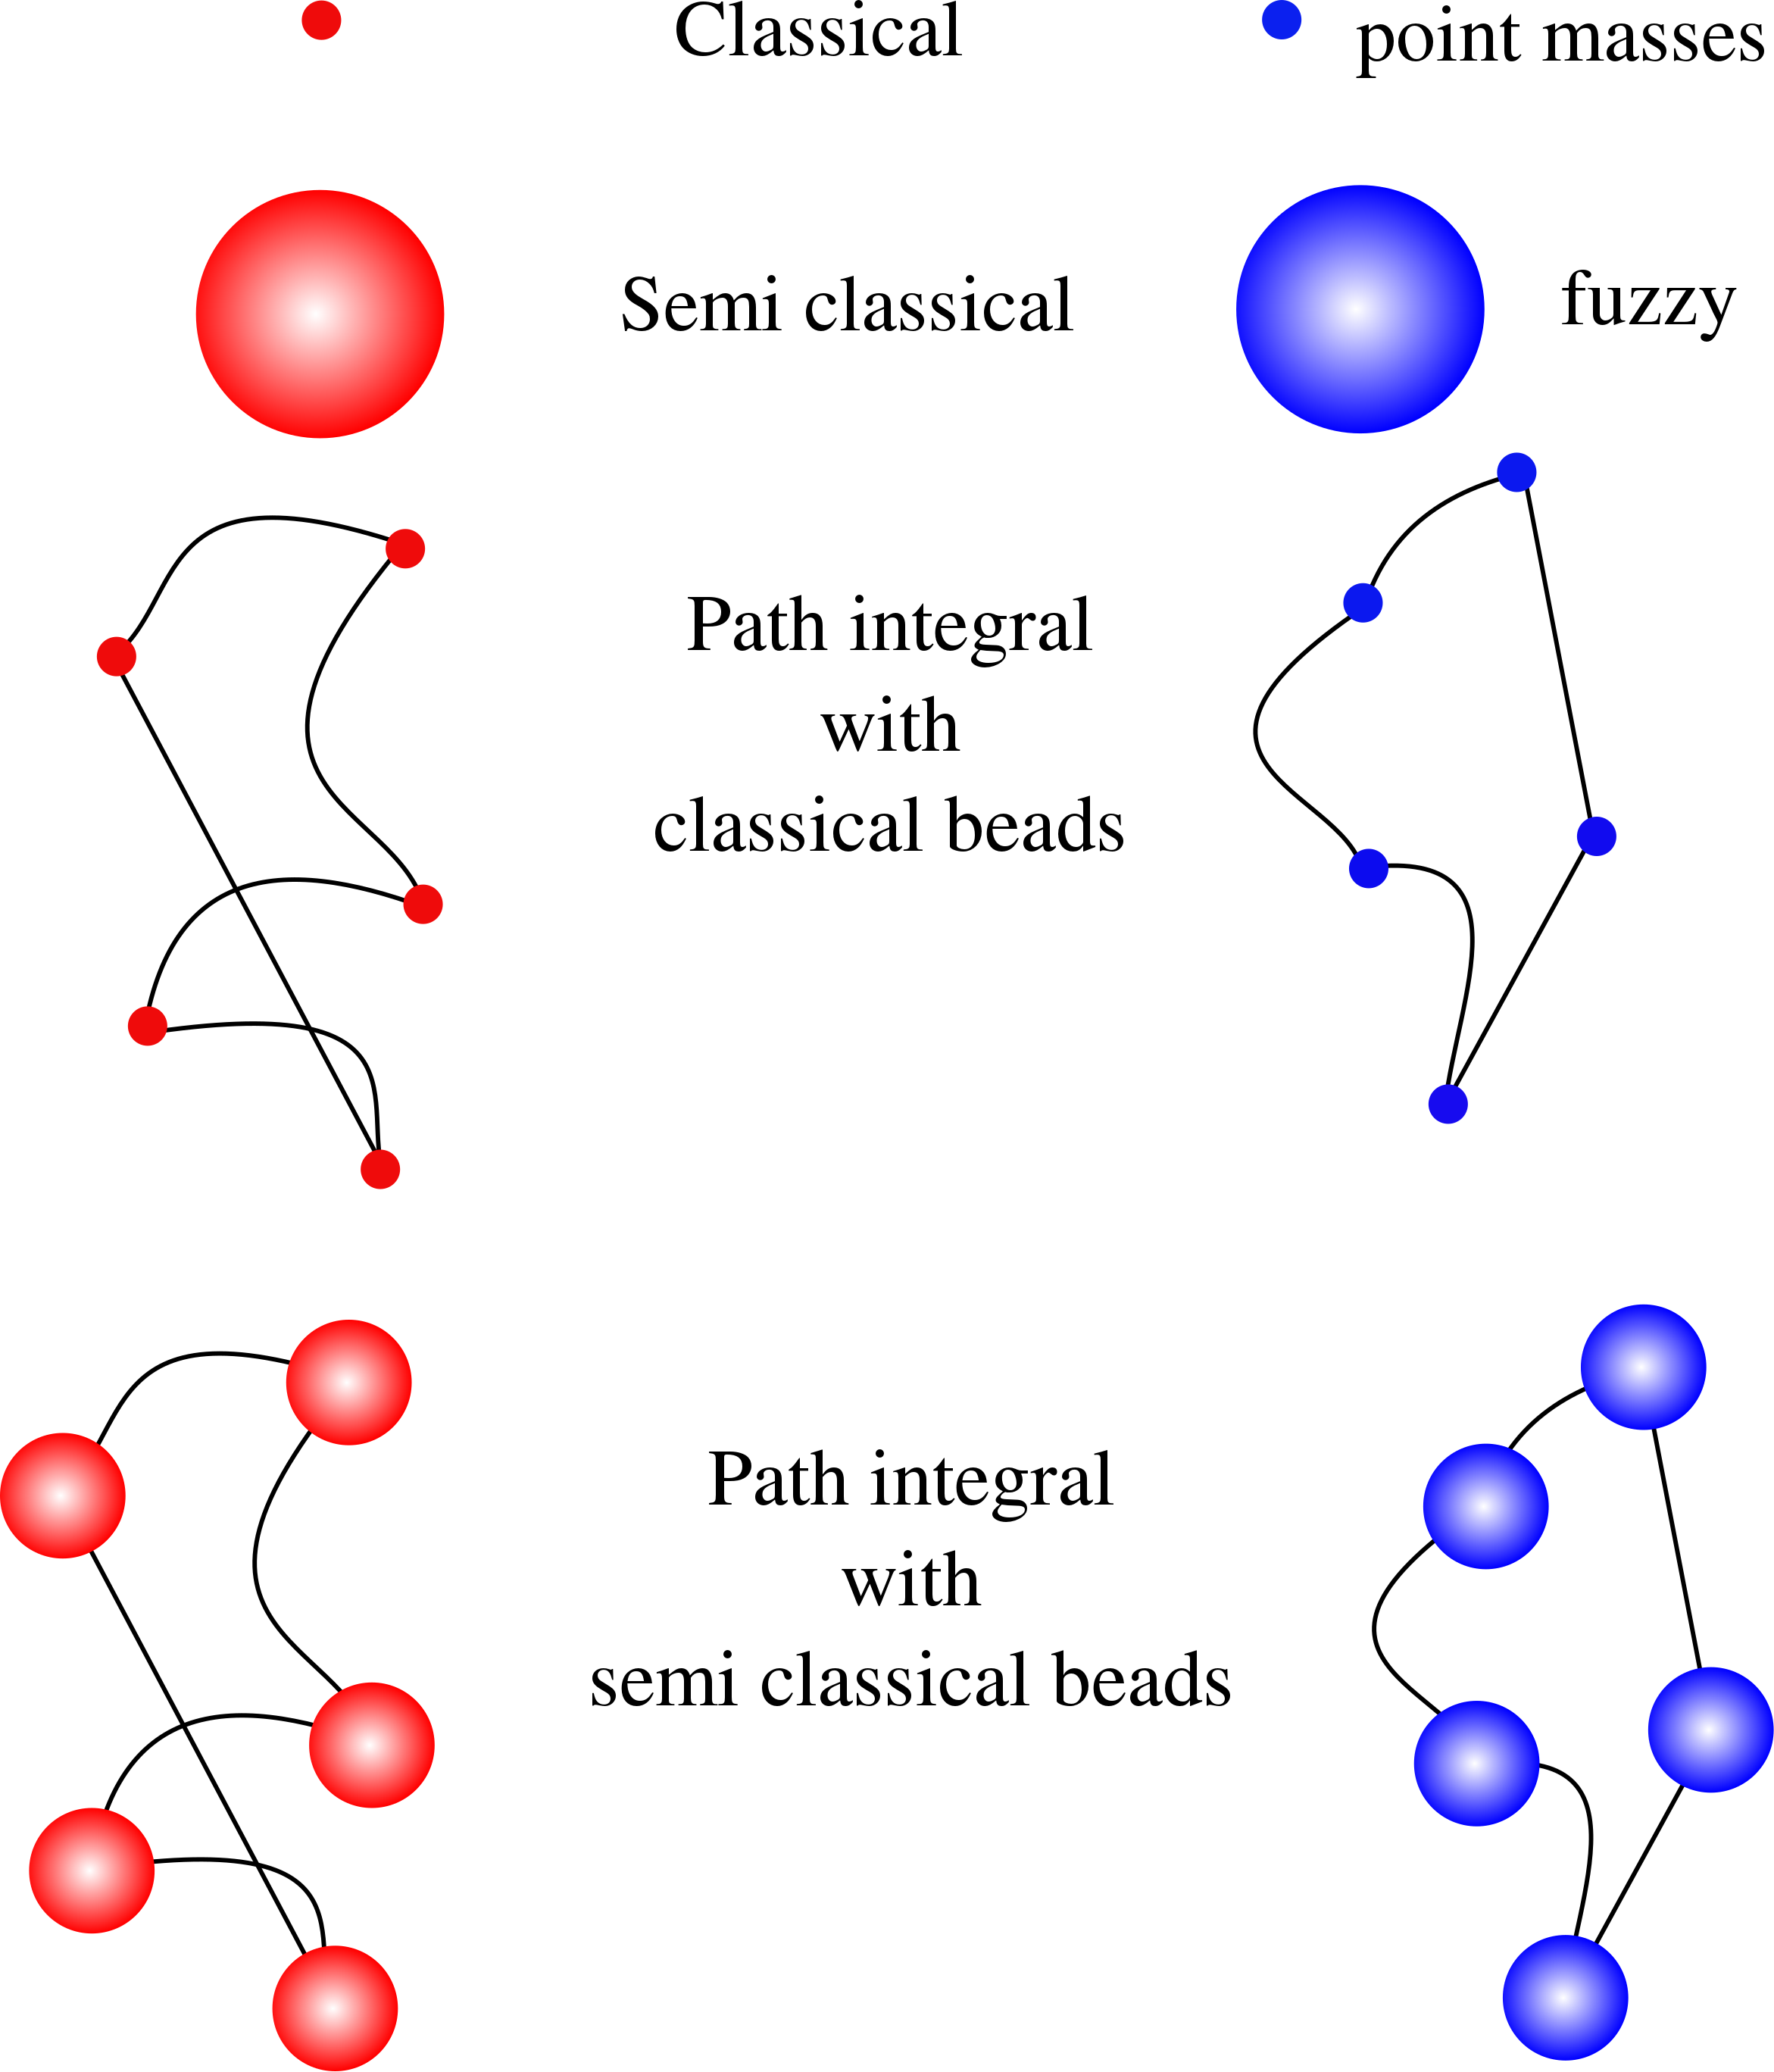
\includegraphics[scale=0.087,keepaspectratio]{quantumLevels.png}
            \caption{Different levels of ``quantumness'' of a $B_2$ calculation going from classical virial coefficients that are calculated assuming point masses to fully quantum virial coefficients with semi-classical beads. The different sphere sizes here are for illustrative purposes only and no quantitative inference should be made.} \label{quantumness}
        \end{figure}
        
        We summarize here the equations pertaining to PIMC calculations with semi-classical beads (SCB) based approach using the TI propagator.
        The fully quantum second virial coefficient expression using SCB-TI approach is given by:
        \begin{equation}
        \label{eq:b2SCBTI}
            B_2 (T) = -2 \pi \displaystyle\int dr~ r^2 (e^{-\beta \bar{U} (r)} - 1)
        \end{equation}
        where $\bar {U} (r)$ is defined for the monatomic case as:
        \begin{equation}
            \label{eq:uBarMonatomicSCBTI}
            \exp [-\beta \bar{U} (|\mbf{r}|) = \left< \exp \left[ -\displaystyle\frac{\beta}{P} \sum_{i=1}^P \mc{V'} (|\mbf{x}^i|) \right] \right>_F
        \end{equation}
        and for the diatomic case as:
        \begin{equation}
            \label{eq:uBarDiatomicSCBTI}
            \exp [-\beta \bar{U} (|\mbf{r}|) = \left< \exp \left[ -\displaystyle\frac{\beta}{P} \sum_{i=1}^P \mc{V'} (|\mbf{x}^i|,\Omega_1^i,\Omega_2^i) \right] \right>_{F,\varrho}
        \end{equation}
        where
        \begin{equation}
        \tag{\eqref{eq:TIworking} revisited}
            \mc{V'} = V (\bm{r}_1, \ldots ,\bm{r}_N) + \frac{\hbar^2}{24m} \bigg(\frac{\beta}{P} \bigg)^2 \displaystyle\sum\limits_{i=1}^N \big|\pmb{\nabla}_i V (\bm{r}_1, \ldots ,\bm{r}_N) \big|^2,
        \end{equation}

    \section{Development of Novel Algorithms}
    \label{sec:novel algorithms}
        Sampling of configurations in PIMC is made difficult by the different range of motions needed for rearrangements of the ring of beads, versus its translation as a whole. This can be alleviated by using Monte Carlo trials having different step sizes or collective moves, but still, the amount of sampling needed for ring arrangements to decorrelate limits the capabilities of these methods. Consequently, special methods have been introduced to speed up this sampling process. For monatomic molecules (e.g., He) only molecular positions are required to be sampled, and the algorithm \cite{Fosdick:1966vh,Patkowski2008,Shaul2012} to accomplish this efficiently is established. It is possible to solve analytically for the probability distribution of the location of each bead in a chain or ring of harmonically interacting beads, and this probability can be used to regrow the ring, or part of it, directly. The acceptance of proposed rearrangement generated this way depends only on the interaction of the beads with other bead-rings in the system. Each accepted trial then yields a new internal arrangement that is uncorrelated from the one that preceded it.

        Going from monatomic to diatomic molecules, rotational and vibrational degrees of freedom add more complexity to the computation and the sampling problem. To start, one can treat the molecule as a quantum-mechanical rigid rotor. Within this approximation there are multiple ways to still accommodate the vibrational degree of freedom (if using a potential model that includes it), and how it is affected by temperature \cite{Garberoglio2012,Garberoglio2014}. Regardless, the monatomic path-integral framework is extended for the rigid rotor by adding an orientational degree of freedom to each bead, coupled to the orientations of adjacent beads in the chain in the manner first described by Cui et al. \cite{Cui1997}. Sampling of positions of the beads can be decoupled from their orientations, so extension of PIMC to the diatomic can focus on finding an efficient way to sample the chain of rotors.  The interactions are not harmonic, so the probability distribution of the chain cannot be determined exactly. Garberoglio and Johnson \cite{Garberoglio2010} introduced a method to sample the path-integral degrees of freedom, based on a hybrid MC method for path integrals that uses molecular dynamics with large time steps \cite{Tuckerman:1993hu}.  This method is used to generate a reservoir of ideal-gas configurations to be used as trials in a larger MC calculation of virial coefficients (or other quantities).

        It is difficult to advance to a full path-integral treatment of rotation and vibration while remaining in the framework of rovibrational quantum states for the diatomic, and even if this were tractable, it does not provide a viable route to extending to multiatomic (more than 2-atom) molecules. A step toward overcoming this problem was made by Garberoglio et al. \cite{Garberoglio2014} in their path-integral treatment of the flexible diatomic. They describe the diatomic molecule by using two independent (albeit bonded) atoms instead of one quantum rigid rotor. This eliminates the need for evaluation of rotational and/or vibrational energy levels, and replaces it with a straightforward path-integral treatment of monatomic entities. In the case of $^4$He \cite{Shaul2012}, it was found that completely regrowing the ring for each MC move was more efficient than applying random displacements to each of the beads. One should expect this to be so \emph{a foritori} for the case of multiatomics. Garberoglio et al. \cite{Garberoglio2014} use the ideal-gas hybrid MC method to generate configurations for sampling in the MC calculation of the second virial coefficient.

        We begin by listing the key equations used for the calculation of the second virial coefficient. We assume throughout a homonuclear dimer, with each atom of mass $m$. The formulas presented here parallel those given by Garberoglio et al. \cite{Garberoglio2014}, who provide a much more detailed development than attempted here. While we follow closely the notation given in Ref. \cite{Garberoglio2014}, there are small differences in some of the definitions, resulting from our choice of a different coordinate system.

        The path-integral formulation represents each atom with $P$ beads, arranged in a closed chain such that each bead interacts with the two beads adjacent to it in the chain, according to a harmonic potential that results from discretizing the kinetic energy term in the action \cite{Feynman}. We shall use the term `image' to denote the set of two beads that make up the diatomic molecule at any point in this chain. The beads may be joined in a Boltzmann (one $P$-bead ring for each atom) or exchange (one $2P$-bead ring encompassing both atoms) conformation.

        The expression we evaluate for the second virial coefficient is \cite{Garberoglio2014}:
        \begin{equation}
        \label{eq:B2}
            B_2(T) =  - \frac{1}{2}\sum\limits_{\sigma ,\sigma '} \int \,d \mbf{Z}^{(1)} d\,\mbf{Z}^{(2)} \Pi _\sigma (\mbf{Z}^{(1)}) \Pi _{\sigma '}(\mbf{Z}^{(2)}) \left( e^{ - \beta \bar U(\mbf{Z}^{(1)} , \mbf{Z}^{(2)}) - 1} \right).
        \end{equation}
        In this formula, $\mbf{Z}^{(i)}$ represents the coordinates of the path-integral beads for the two atoms in molecule $i$, and
        $\Pi_\sigma(\mbf{Z}^{(i)})$ is the ideal-gas weight for molecule $i$ in configuration $\mbf{Z}^{(i)}$:
        \begin{equation}
        \label{eq:weight}
            \Pi _\sigma (\mbf{Z}) = \frac{\delta _{\sigma ,{\rm B}} Q_1^{({\rm B})} P_B (\mbf{Z}) + \delta _{\sigma ,{\rm xc}} Q_1^{({\rm xc})} P_{\rm xc} (\mbf{Z})} { Q_1^{({\rm B})} + Q_1^{({\rm xc})}}
        \end{equation}
        The subscript $\sigma$ indicates whether the beads are in a Boltzmann (``B'') or exchange (``xc'') conformation; intermolecular exchange is neglected. Whereas in Ref. \citenum{Garberoglio2014} the atom positions were represented by their respective Cartesian coordinates, in the present work we represent them in terms of their $P$ molecule centers $\mbf{R}$ and $P$ atom-separation vectors $\mbf{b}$, such that the positions of the two atoms on molecule $i$ are $\mbf{R}_i+\mbf{b}_i/2$ and $\mbf{R}_i-\mbf{b}_i/2$, respectively; thus, $\mbf{Z} = (\mbf{R},\mbf{b})$.

        The images are labeled sequentially from 0 to $P$, and we distinguish the Boltzmann versus exchange cases via the interpretation of the orientation of image $P$: for the Boltzmann case, $\mbf{b}_P = \mbf{b}_0$, while in the exchange case $\mbf{b}_P = -\mbf{b}_0$. By applying this interpretation throughout the development, we can present both cases using a common set of formulas and algorithms. We will use the notation $\mbf{b}^{(\sigma)}$ to represent the set of $\mbf{b}$ vectors where the distinction between Boltzmann and exchange is relevant; otherwise we will represent the set simply as $\mbf{b}$.

        In Eq.~\ref{eq:weight}, ${P_\sigma}(\mbf{Z})$ is the probability of configuration $\mbf{Z}$ given that the ring is in a Boltzmann or exchange arrangement, respectively:
        \begin{equation}
        \label{eq:PIProb}
            P_\sigma (\mbf{Z}) = \frac{1}{Q_1^{{\rm (\sigma)}}} F(\mbf{R};2m) F(\mbf{b}^{(\sigma)};m/2) e^{ - \beta \bar u(\mbf{b})}
        \end{equation}
        where $F$ is the path-integral weight, and $\bar u$ is the intramolecular potential energy averaged over all images:
        \begin{equation}
            \begin{aligned}
                F(\mbf{x};m) &= \left( \frac{P^{3/2}} {\Lambda _m^3} \right)^P \exp \left[ - \frac{\pi P}{\Lambda _m^2}\sum\limits_{i = 0}^{P-1} \left| \mbf{x}_{i + 1} - \mbf{x}_i \right|^2 \right]\\
                &\bar u(\mbf{b}) = \frac{1}{P}\sum\limits_{i=0}^{P-1} {u\left(b_i \right)} \nonumber\\
                &\Lambda_m=\frac{h}{\sqrt{2\pi m k_{\rm B}T}}\nonumber
            \end{aligned}
        \end{equation}
        where $b_i \equiv \left| \mbf{b}_i \right|$. We also have in Eqs. \ref{eq:weight} and \ref{eq:PIProb} the 1-molecule partition function for the Boltzmann and exchange cases:
        \begin{equation}
        \label{eq:Q1}
            \begin{aligned}
                Q_1^{({\rm \sigma})} &= \int d\mbf{Z} F(\mbf{R};2m)F(\mbf{b}^{(\sigma)};m/2) e^{ - \beta \bar u(\mbf{b})}\nonumber\\
                &=\frac{1}{\Lambda_{2m}^3}\int d\mbf{b}F(\mbf{b}^{(\sigma)};m/2) e^{ - \beta \bar u(\mbf{b})}
            \end{aligned}
        \end{equation}
        As discussed in \cite{Garberoglio2014}, the integrals defining $Q_1$ are taken over all $2P$ atom bead coordinates except one, which is fixed at the origin. Likewise, the coordinates of one of the $4P$ atom bead coordinates in the integral for $B_2$ in Eq.~\ref{eq:B2} is fixed, and defines the origin. With these stipulations, terms proportional to the system volume $V$ cancel each other (assuming $V$ is large), and the coefficient $B_2$ is volume-independent.

        Finally, in Eq.~\ref{eq:B2} there is $\bar U$, the intermolecular potential energy averaged over all $P$ interacting images:
        \begin{equation}
            \bar U\left( \mbf{Z}^{(1)}, \mbf{Z}^{(2)} \right) = \frac{1}{P}\sum\limits_{i = 0}^{P-1} U\left( \mbf{Z}_i^{(1)},\mbf{Z}_i^{(2)} \right)
        \end{equation}

        The general approach taken to the calculation of $B_2$ is to sample the position of molecule 2 using a Mayer-sampling scheme \cite{Singh2004}, while sampling of orientations and internal conformations of the path-integral rings of both molecules is accomplished through direct sampling of each dimer independently. With knowledge of the ratio $Q_1^{\rm (xc)}/Q_1^{\rm (B)}$ it is a simple matter to sample the exchange-versus-Boltzmann coordinate $\sigma$. For each case, the target distribution for the ring conformation, $P_\sigma(\mbf{Z})$, factors cleanly into a component that depends on only the molecule-center coordinates $\mbf{R}$, and another depending only on the intramolecular coordinates $\mbf{b}$. The molecule-center distribution is just a ring of Gaussians in 3D space, and these can be sampled directly. Specifically, with $\mbf{R}_1$ at the origin, each image coordinate $\mbf{R}_i$ is sampled in sequence from a Gaussian of standard deviation $\sigma_i$ in each dimension centered at a position $\mbf{R}_i'$, such that \cite{Shaul2012}
        \begin{equation}
            \begin{aligned}
                \sigma _i &= \left( \frac{\Lambda _{2m}^2}{2\pi P}\;\frac{P + 1 - i}{P + 2 - i} \right)^{1/2},\\
                \mbf{R}_i'  &= \frac{P + 1 - i}{P + 2 - i}{\mbf{R}_{i - 1}};
            \end{aligned}
        \end{equation}
        for molecule 2, the ring constructed in this manner is then translated to its position specified by the larger Mayer-sampling process.

        This leaves sampling of the intramolecular coordinates $\mbf{b}$. These coordinates are also distributed as a ring (for Boltzmann) or chain (for exchange) of Gaussians, but constrained by the intramolecular potential $\bar u(\mbf{b})$, which makes the problem of exact direct sampling intractable in general. For a target distribution $\pi_\sigma(\mbf{b})$, defined as the $\mbf{b}$-dependent terms in Eq.~\ref{eq:PIProb} for $P_\sigma$, we can instead sample according to an approximate distribution $\tilde \pi_\sigma(\mbf{b})$, constructed so it can be sampled directly. We use a configuration sampled on this distribution to generate a Monte Carlo trial, which we accept or reject based on the acceptance probability $P_{\rm acc}$ as:
        \begin{equation}
        \label{eq:Pacc}
            P_{\rm acc} = \frac{\pi^{\rm new}/\pi^{\rm old}}{\tilde \pi^{\rm new}/\tilde \pi^{\rm old}}
        \end{equation}
        where the superscripts denote the old and new configurations respectively.

        We next describe an algorithm to generate configurations according to an approximate distribution $\tilde\pi(\mbf{b}^{(\sigma)})$. We do this first for the case of a rigid diatomic, with atoms separated by a fixed bond length, and then develop the approach for the case of a fully flexible diatomic.
    \subsection{Orientation Sampling Algorithm}
    \label{subsec:orMove}
        We employ a bisection approach to generate a chain or ring of image orientations with a probability distribution that approximates $\pi(\mbf{b}^{(\sigma)})$. At each step in the process, we are given orientations of two images, $\mbf{b}_i$ and $\mbf{b}_k$, and we aim to generate an orientation for another image $\mbf{b}_j$, $j = (i+k)/2$, that is approximately consistent with $\pi(\mbf{b}^{(\sigma)})$ for the given image orientations. Then in the subsequent step we generate an orientation for an image halfway between $i$ and the new $j$ image, and again between $j$ and $k$. This process repeats until all images are assigned orientations. For the end case, where $j = i+1 = k-1$, we are able to select a $\mbf{b}_j$ that is exactly as prescribed by $\pi(\mbf{b}^{(\sigma)})$ given the previously-assigned orientations. For the steps preceding this one, in which other images are to be subsequently inserted between $j$ and $i$ and between $j$ and $k$, we can do this only approximately. To facilitate this process, we work with numbers of images $P = 2^n$, where $n$ is an integer; then in this scheme, half of the images ($2^{n-1}$) are oriented to follow $\pi(\mbf{b}^{(\sigma)})$ exactly, and the other half are placed to follow it approximately.

        Let us first examine the end case, in which an image orientation is selected, given the orientation of its two adjacent neighbors in the chain. Consider a sphere of \emph{diameter} equal to the molecule bond length $b$ (assumed to be the same for all images). One may think of the orientation vector $\mbf{b}_j/2$ as locating an orientation bead on the surface of the sphere, which interacts with adjacent orientation beads---also on the sphere---with a harmonic potential defined in terms of their Euclidean distance, such that they contribute to the configuration weight by a factor
        \ifkhExplicitP
            \begin{equation}
            \label{eq:piRigid}
                \begin{aligned}
                    \pi(\mbf{b}_i,\mbf{b}_j) &= \exp\left(-k_h |\mbf{b}_i - \mbf{b}_j|^2/b^2\right)\\
                    k_h &=\frac{\pi P b^2}{\Lambda^2_{m/2}}\nonumber
                \end{aligned}
            \end{equation}
        \else
            \begin{equation}
            \label{eq:piRigid}
                \begin{aligned}
                    \pi(\mbf{b}_i,\mbf{b}_j) &= \exp\left(-k_h |\mbf{b}_i - \mbf{b}_j|^2\right)\\
                    k_h &=\frac{\pi P}{\Lambda^2_{m/2}}\nonumber
                \end{aligned}
            \end{equation}
        \fi
        so that, in accord with Eq.~\ref{eq:PIProb} with the rigid bond constraint imposed in lieu of the intramolecular energy term,
        \begin{equation}
        \label{eq:piTotal}
            \pi(\mbf{b}^{(\sigma)}) = \prod_{i=0}^{P-1}\pi(\mbf{b}_i,\mbf{b}_{i+1}).
        \end{equation}
        \ifkhExplicitP
            We note that $k_h$ is dimensionless, and for H$_2$ is about xxx.
        \else
            We note that the unit of $k_h$ is \AA$^{-2}$.
        \fi

        In order to express $b^2_{ij} \equiv |\mbf{b}_i - \mbf{b}_{j}|^2$ in terms of angles, consider the orientations of image $i$ and image $k$ as indicated by A and B respectively in Fig. \ref{fig:simple}, with $\angle AOB = \psi$. Let $\mathbf a$ be the vector bisecting $\mbf{b}_i$ and  $\mbf{b}_k$. By $\tilde \pi(\mbf{b}_j: \mathbf{a}, \alpha, \beta)$ we denote the probability distribution centered around $\mathbf a$, of generating a configuration for orientation image $j$ (indicated by C, and the angles $\alpha$ and $\beta$ in Fig. \ref{fig:simple}).
        \begin{figure}[!htbp]
            \centering
            \def\svgwidth{0.25\columnwidth}
            \input{Chapter-2/Figures/distanceNew1.pdf_tex}
            \caption{Simplified picture}
            \label{fig:simple}
        \end{figure}
        Using basic coordinate geometry and trigonometric relations, the following expressions for the various distances can be easily obtained (see Appendix \ref{Appendix A} for complete mathematical details):
        \begin{equation}
        \label{eq:deltax}
            \begin{aligned}
                d_{AC}^2 &= \frac{b^2}{2} [1 - \cos(\psi/2) \cos(\alpha) + \sin(\psi/2) \sin(\alpha) \cos(\beta)]\\
                d_{BC}^2 &= \frac{b^2}{2} [1 - \cos(\psi/2) \cos(\alpha) - \sin(\psi/2) \sin(\alpha) \cos(\beta)]
            \end{aligned}
        \end{equation}

        The total weight for the orientation $j$ is then calculated as \footnote{Note that in Eq. \eqref{eq:Uh} $|\mbf{b}_i - \mbf{b}_j|^2 + |\mbf{b}_j - \mbf{b}_k|^2 = 4 (d_{AC}^2 + d_{BC}^2)$}:
        \ifkhExplicitP
            \begin{equation}
            \label{eq:Uh}
                \begin{aligned}
                    \tilde \pi(\mbf{b}_j: \mathbf{a}, \alpha, \beta)  &= \pi(\mbf{b}_i,\mbf{b}_j)\pi(\mbf{b}_j,\mbf{b}_k)\\
                    &= \exp\left(-4 k_h [d_{AC}^2 + d_{BC}^2]/b^2\right)\\
                    &= \exp\left(-4 k_h [1 - \cos(\psi/2) \cos(\alpha)]\right)
                \end{aligned}
            \end{equation}
        \else
            \begin{equation}
            \label{eq:Uh}
                \begin{aligned}
                    \tilde \pi(\mbf{b}_j: \mathbf{a}, \alpha, \beta)  &= \pi(\mbf{b}_i,\mbf{b}_j)\pi(\mbf{b}_j,\mbf{b}_k)\\
                    &= \exp\left(-4 k_h [d_{AC}^2 + d_{BC}^2]\right)\\
                    &= \exp\left(-4k_h~b^2 [1 - \cos(\psi/2) \cos(\alpha)]\right)
                \end{aligned}
            \end{equation}
        \fi

        This expression is independent of $\beta$, so we can choose it at random, uniformly on $[0, 2\pi]$. For the special case of $\psi = \pi$ since the r.h.s. of Eq. \eqref{eq:Uh} becomes independent of $\alpha$, we can choose it just like $\beta$, i.e., at random, uniformly on $[0, 2\pi]$. To choose $\alpha$ for all other cases, we first normalize $\tilde \pi(\mbf{b}_j: \mathbf{a}, \alpha, \beta) $ and evaluate a cumulative distribution function $C(\alpha)$ (Eq. \eqref{eq:cdf}), which we then invert to obtain an expression for $\alpha$ (see Appendix \ref{Appendix C} for mathematical details). Selection of $\alpha$ is then made by evaluating this expression with $C$ chosen at random, uniformly on [0,1] as :
        \ifkhExplicitP
            \begin{equation}
            \label{eq:alpha}
                \begin{aligned}
                    \alpha &= \cos^{-1} \left[1 +  (1/\kappa)\ln\left(1 - C (1-\exp[-2\kappa]) \right) \right],\\
                    \text{where}\:\:\: \kappa &= 4 \cos(\psi/2) k_h
                \end{aligned}
            \end{equation}
        \else
            \begin{equation}
            \label{eq:alpha}
                \begin{aligned}
                    \alpha &= \cos^{-1} \left[1 +  (1/\kappa)\ln\left(1 - C (1-\exp[-2\kappa]) \right) \right],\\
                    \text{where}\:\:\: \kappa &= 4 \cos(\psi/2) k_h~b^2
                \end{aligned}
            \end{equation}
        \fi

        We just explained how to choose an orientation for any image $j$ that is adjacent to images $i$ and $k$ (Note: $\tilde \pi (\mbf{b})$ is always equal to $\pi (\mbf{b})$ for this case). Before this step can be taken, $i$ and $k$ must have been placed in a similar fashion. These orientation images do not interact directly, but instead have an effective interaction that can be defined by integration over the $j$ orientation:
        \ifkhExplicitP
            \begin{equation}
            \label{eq:piEff}
                \begin{aligned}
                    \pi^{\rm eff}(\mbf{b}_i,\mbf{b}_k)&= \sin(\psi)\int d\mbf{b}_j \: \: \tilde \pi(\mbf{b}_j: \mathbf{a}, \alpha, \beta) \nonumber \\
                    &=\frac{\pi b}{k_h}\left( e^{ - 8 k_h \sin^2 \left( \frac{\psi}{4}\right)} - e^{ - 8 k_h \cos^2 \left( \frac{\psi}{4} \right)} \right) \sin \left(\psi /2 \right)
                \end{aligned}
            \end{equation}
        \else
            \begin{equation}
            \label{eq:piEff}
                \begin{aligned}
                    \pi^{\rm eff}(\mbf{b}_i,\mbf{b}_k)&= \sin(\psi)\int d\mbf{b}_j \: \: \tilde \pi(\mbf{b}_j: \mathbf{a}, \alpha, \beta) \nonumber \\
                    &=\frac{\pi}{k_h~b}\left( e^{ - 8 k_h~b^2 \sin^2 \left( \frac{\psi}{4}\right)} - e^{ - 8 k_h~b^2 \cos^2 \left( \frac{\psi}{4} \right)} \right) \sin \left(\psi /2 \right)
                \end{aligned}
            \end{equation}
        \fi
        This effective interaction (as manifest via $\psi$) obviously is not a simple harmonic, so  it is difficult to proceed in an exact analytic manner as we did for the adjacent-image case. However, we can perform a second-order series expansion of $\ln \pi^{\rm eff}$ in terms of the $ik$ distance $d_{ik} = 2b\sin(\psi/2)$, to identify an effective harmonic interaction:
        \begin{equation}
            \begin{aligned}
                k_h^{\rm eff} &= \frac{1}{2}k_h\coth(4 k_h)\\
                &\approx \frac{k_h}{2} \qquad (P \gg 1)\nonumber
            \end{aligned}
        \end{equation}
        The approximate value here is the spring constant for the case where $P$ is half of the value used in placing $j$. Equivalently, this is the spring constant used if the number of images were such that $i$ and $k$ were actually the end cases in the process. We can repeat this prescription all the way back through the bisection process. We summarize the bisection algorithm for choosing the image orientations as follows: (1) orient the first image by selecting a point randomly on a sphere; for the Boltzmann case, this represents the first and last image in the ring; for exchange, the last image would be directed opposite to this one; (2) using a value of $k_h$ for $P = 2$, place the next image by sampling as described by Eq.~\ref{eq:alpha} with $\psi = 0$ (Boltzmann) or $\psi = \pi$ (exchange); (3) double $k_h$ and place two more images between the ones set by steps (1) and (2), sampling according to Eq.~\ref{eq:alpha}; (4) repeat the process of doubling $k_h$ and inserting image orientations between the ones placed in the previous steps, until all image orientations are set. The resulting configuration is generated with probability density (see sec. \ref{Appendix C} for further details):
        \begin{equation}
        \label{eq:piTilde}
            \begin{aligned}
                \tilde \pi(\mbf{b}) &= \displaystyle\prod_{j=1}^{P-1} \tilde \pi(\mbf{b}_j: \mbf{a}) \\
                \tilde \pi(\mbf{b}_j: \mbf{a})  &=
                \begin{cases}
                    \displaystyle\frac{\kappa \times \exp[\kappa \cos (\alpha)]}{\exp[\kappa] - \exp[-\kappa]} & \text{if} \qquad \psi \ne \pi\\
                    \displaystyle\frac{1}{2 \pi b} & \text{if} \qquad \psi = \pi\\
                \end{cases}
            \end{aligned}
        \end{equation}
        It is straightforward to see that the ratio of the approximate and actual probability distribution of $\alpha$ will differ from unity the most for the first step, and gradually improve until the last step, where the two probabilities are equal (given the placement of the other orientations) . The overall percentage of moves accepted will be related to the product of such ratios. Hence, it can be clearly seen that the performance of the algorithm will decrease with increasing $P$ (the accuracy of the result is however unaffected by this).
    \subsection{Bond Length Sampling Algorithm}
    \label{subsec:blMove}
        The method we use to generate configurations for flexible diatomics builds on the scheme described above for rigid molecules. In one type of MC trial, we generate the orientations of the images using the algorithm described above, leaving the bond lengths unchanged. However, that orientation-sampling method is developed assuming all bond lengths are equal, but in the case of flexible molecules, they of course differ. We examined different schemes to handle flexibility within the orientation move. The method we use is to average the bond lengths of images $i$ through $k$ before each orientation move and use this value for image $j$ when setting the new orientation. Although we generate orientations assuming a common bond length for images $i$ through $k$, none of the image bond-lengths are changed by the trial.

        A separate MC trial is used to change the bond lengths, which is performed all at once for all images. With the orientations set, the distribution of bond lengths can be written
        \begin{equation}
            \begin{aligned}
                \pi(\mathbf{b}) &= \displaystyle\prod\limits_{i=0}^{P-1} b_i^2 e^{-\beta u(b_i)/P} \pi(b_i,b_{i+1},\theta_{i,i+1}) \\
                \pi(b_i,b_j,\theta_{i,j}) &= \exp\left(-\frac{1}{2}  k_h  \left( b_i^2 + b_j^2 - 2  b_i  b_j  \cos (\theta_{ij}) \right)\right)\\
            \end{aligned}
        \end{equation}
        where $\theta_{i,j}$ is the angle between orientations of images $i$ and $j$, with $\theta_{P-1,P}$ defined using the convention described above for Boltzmann versus exchange configurations.
        We can clearly see that $\pi(\mathbf{b})$ is not Gaussian, and the $P$ $b$-values are coupled and hence not easy to sample directly. We formulate an approximate sampling scheme by introducing a Gaussian approximation, which through a normal-mode calculation we can sample directly (see Appendix \ref{Appendix B} for mathematical details). However, it would be unnecessarily expensive computationally to perform the normal-mode analysis before each bond length move, so instead we define the normal modes for a given $P$ using a single representative angle $\hat \theta$ for all $ij$ pairs. Then the normal-mode analysis need be performed only once, at the beginning of the simulation.

        Let $\pi(\mathbf{b}) = $~$ \exp (-y)$, where $y$ can be defined as follows:-
        \begin{equation}
        \label{eq:y}
            \begin{aligned}
                y &= -\ln \pi(\mathbf{b})\\
                y &= \displaystyle\sum\limits_{i=0}^{P-1} \Bigg\{ \frac{1}{2}  k_h  \Big( b_i^2 + b_j^2 - 2  b_i  b_j  \cos (\theta_{ij}) \Big) - 2  \log b_i + \frac{ \beta  u (b_i)}{P} \Bigg\}\\
                &= \displaystyle\sum\limits_{i=0}^{P-1} \Bigg\{ k_h  \Big( b_i^2 - b_i  b_j  \cos (\theta_{ij}) \Big) - 2  \log b_i + \frac{ \beta  u (b_i)}{P} \Bigg\}
            \end{aligned}
        \end{equation}

        To compute a nominal value for this angle, we first assume that the orientations of all images are the same or in other words $\theta_{ij} = 0$. From eq. \eqref{eq:y}, we can see that there are two terms that are negative, the term containing $\cos (\theta_{ij})$ and the term containing $\log b_i$. Assuming we take the common negative sign out, since we are setting $\cos (\theta_{ij})$ to its maximum value 1 thereby increasing the first term, we need to reduce the second term to balance out this effect. In other words, the effect of different images having different orientations is accounted for, by using the term $b_i^{2/P}$ instead of $b_i^2$ in the expression for $y$. This gives us a new definition for $\tilde y$ as:
        \begin{equation}
        \label{eq:ytilde}
            \begin{aligned}
                \tilde y &\approx y\\
                \tilde y &= \displaystyle\sum\limits_{i=0}^{P-1} \Bigg\{ k_h  \Big( b_i^2 - b_i  b_j \Big) - \frac{2  \log b_i}{P} + \frac{ \beta  u (b_i)}{P} \Bigg\}
            \end{aligned}
        \end{equation}

        It should be noted that the term $b_i^{2/P}$ has no physical meaning whatsoever and it was artificially introduced solely to account for different images having different orientations (see sec. \ref{sec:blPerformance} for justification of this approach). We solve for the nominal $\cos (\hat \theta)$ value by setting the first derivatives of $y$ and $\tilde y$ equal and get:
        \begin{equation}
        \label{eq:thetaHat}
            \cos (\hat \theta) = 1 - \frac{P-1}{P~k_h~b_i^2}
        \end{equation}

        Using this nominal value in Eq. \eqref{eq:y}, we find $b_m$ such that:
        \begin{equation}
        \label{eq:bm}
            \displaystyle\frac{\partial y}{\partial b_i} \bigg|_{b_i = b_m} = 0 \qquad \forall i
        \end{equation}

        We employ Newton-Raphson method to compute $b_m$ and use it to perform the normal mode analysis only once for a simulation. It is worth noting that here too, like the orientation move, we have used an approximate distribution function to choose the different bond lengths. Therefore, much like the orientation move, the performance of the algorithm is expected to decrease with increasing $P$.
